% Fig. 3.22 -- the range of (U, V) drawn twice: once in the original
% (x_1, x_2) plane with the boundaries of U marked on it, and once in the
% (v, u) plane the change of variables carries it to.
% Source: mathstatch3.tex lines 4904-4958 (left panel) and 4961-4998 (right
% panel), two tikzpictures set side by side in minipages of .58 and .40 of
% the text width, both at scale=0.75.
%
% Every element of both manuscript panels is kept.  Upper panel: the shaded
% unit square with its top and right edges outlined, the line u = 0 drawn
% over -1/3 <= x_1 <= 1/3, the line u = 2 drawn over 2/3 <= x_1 <= 4/3, the
% dashed line u = 1 from (0,1) to (1,0), and the five marks 0, 1, 1, x_1 = v
% and x_2.  Lower panel: the shaded parallelogram (0,0), (1,1), (1,2), (0,1),
% the two boundary lines v = u and v = u - 1 drawn over -1/6 <= v <= 7/6, the
% solid segment v = 1 between u = 1 and u = 2, the three dashed guides, and
% the marks 0, 1, 2, 1, v and u.  Manuscript colours (gray at opacity 0.2,
% black) give way to the palette of CH3_FIGURE_SPECS.md section 1.
%
% Three departures from the manuscript, all forced by the web setting:
%
% 1. The panels are stacked rather than set side by side.  Their figure
%    column is 268px on a 390px phone (a topic-figure inside a Note box that
%    is itself inside an Example box), and side by side each panel would get
%    about 130px, far too little for labels such as u = x_1 + x_2 = 2.  The
%    stacked arrangement follows convexity-tangent-lines.tex and
%    jensen-inequality.tex.  Both panels keep one common unit length, so the
%    unit square of the upper panel and the parallelogram of the lower one
%    can be compared side lengths and all.
%
% 2. The manuscript's connecting arrow \xRightarrow{令 u=x_1+x_2, v=x_1} runs
%    left to right and carries a Chinese character.  Stacked panels need a
%    downward arrow, and CH2_FIGURE_SPECS.md 1.4 bars Chinese from inside the
%    picture, so the arrow is a plain \Downarrow with the two substitutions
%    written beside it.
%
% 3. The axis names $x_1 = v$, $x_2$, $v$ and $u$ sit at 4.5 and 4.3 in the
%    manuscript while the axes stop at 3.8, so each floats clear of its arrow
%    head; here each sits against its own head, per CH2_FIGURE_SPECS.md 1.3.
%
% \DeclareMathSizes{12}{12}{10}{9} lifts the math script size from the 8.5pt
% default: the subscripts of x_1 and x_2 are the smallest marks in the
% picture and would otherwise fall under the floor.
%
% Native size 219.204 x 381 pt.  A mark of S pt shows at
% S x 0.99626 x <display width> / 219.204 px, so at the 268px phone column
% and the 460px desktop column of a topic-figure--medium in that doubly
% nested box:
%     10pt scripts  12.18px (phone)   20.91px (desktop)
%     12pt text     14.62px (phone)   25.09px (desktop)
% At the nominal 350px of the ledger convention the scripts stand at 15.91px.
\documentclass[tikz,border=2pt]{standalone}
\usepackage{amsmath}
\usepackage{amssymb}
\usepackage{xcolor}

\definecolor{journalink}{HTML}{1F1C18}
\definecolor{journalmuted}{HTML}{8A7F72}
\definecolor{journalaccent}{HTML}{9C2D2D}

\DeclareMathSizes{12}{12}{10}{9}

\begin{document}
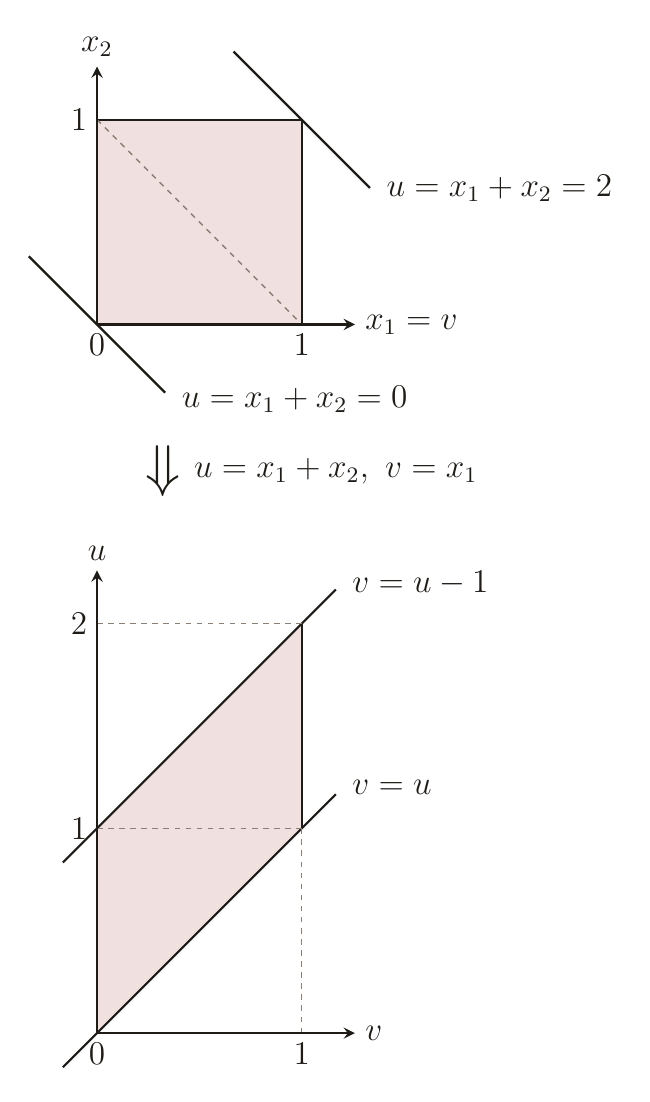
\begin{tikzpicture}[x=2.6cm, y=2.6cm, >=stealth,
                    every node/.style={journalink, font=\large}]

%% ==== 上面板: 轉換之前的 (x_1, x_2) 平面 ============================
\begin{scope}

  %% 聯合值域: 單位正方形
  \fill[journalaccent, fill opacity=0.15] (0,0) rectangle (1,1);

  \draw[journalink, line width=0.8pt] (0,1) -- (1,1);
  \draw[journalink, line width=0.8pt] (1,0) -- (1,1);

  %% u = x_1+x_2 = 1 這條線, 書稿畫成虛線
  \draw[journalmuted, line width=0.5pt, dash pattern=on 2pt off 2pt]
    (0,1) -- (1,0);

  %% u 的兩個端點所對應的兩條線
  \draw[journalink, line width=0.8pt] (-0.33333,0.33333) -- (0.33333,-0.33333);
  \draw[journalink, line width=0.8pt] (0.66667,1.33333) -- (1.33333,0.66667);

  %% 座標軸
  \draw[journalink, line width=0.8pt, ->] (0,0) -- (1.26,0) node[right] {$x_1=v$};
  \draw[journalink, line width=0.8pt, ->] (0,0) -- (0,1.26) node[above] {$x_2$};

  %% 刻度標示
  \node[below] at (1,0) {$1$};
  \node[below] at (0,0) {$0$};
  \node[left]  at (0,1) {$1$};

  %% 兩條線各自的方程式
  \node[right] at (0.36667,-0.36667) {$u=x_1+x_2=0$};
  \node[right] at (1.36667,0.66667)  {$u=x_1+x_2=2$};

\end{scope}

%% ==== 轉換 ==========================================================
\node[font=\huge] at (0.321,-0.7173) {$\Downarrow$};
\node[right] at (0.427,-0.7173) {$u=x_1+x_2,\ v=x_1$};

%% ==== 下面板: 轉換之後的 (v, u) 平面 ================================
\begin{scope}[yshift=-9.0cm]

  %% (U, V) 的聯合值域: 0<v<1 且 v<u<v+1 的平行四邊形
  \fill[journalaccent, fill opacity=0.15] (0,0) -- (1,1) -- (1,2) -- (0,1) -- cycle;

  %% 兩條邊界 v = u 與 v = u-1
  \draw[journalink, line width=0.8pt] (-0.16667,-0.16667) -- (1.16667,1.16667);
  \draw[journalink, line width=0.8pt] (-0.16667,0.83333) -- (1.16667,2.16667);

  %% 邊界 v = 1
  \draw[journalink, line width=0.8pt] (1,1) -- (1,2);

  %% 輔助虛線
  \draw[journalmuted, line width=0.5pt, dash pattern=on 2pt off 2pt] (0,1) -- (1,1);
  \draw[journalmuted, line width=0.5pt, dash pattern=on 2pt off 2pt] (0,2) -- (1,2);
  \draw[journalmuted, line width=0.5pt, dash pattern=on 2pt off 2pt] (1,0) -- (1,1);

  %% 座標軸
  \draw[journalink, line width=0.8pt, ->] (0,0) -- (1.26,0) node[right] {$v$};
  \draw[journalink, line width=0.8pt, ->] (0,0) -- (0,2.26) node[above] {$u$};

  %% 刻度標示
  \node[below] at (1,0) {$1$};
  \node[below] at (0,0) {$0$};
  \node[left]  at (0,1) {$1$};
  \node[left]  at (0,2) {$2$};

  %% 兩條邊界各自的方程式
  \node[right] at (1.2,2.2) {$v=u-1$};
  \node[right] at (1.2,1.2) {$v=u$};

\end{scope}

\end{tikzpicture}
\end{document}
